\chapter{Analysis Of Existing models}

As said before, drone swarms are governed by these models mobility. Our study of existing models is therefore divided into several parts.

\section{Summary of the problem}

The issue of this paper is to scan an area as efficiently as possible and as quickly as possible, at least once per hour. This area will be scanned by a UAV swarm that will cooperate and communicate together.

\section{Existing models}

Many mobility models exist with different characteristics. All these models are used to define movements for swarm of UAV. Most models are based on real-life situations such as road maps, or on the behavior of many animals (ants, birds, termites, wolves etc). We will expose some of them we consider the most important and most interesting for our case.

\newpage

\subsection{Random Walk}

First described by Einstein in 1926, it was developed to mimic the extremely unpredictable movement of many entities in nature. A mobility node (MN) moves from its position to a new one by randomly choosing a direction and speed chosen by pre-defined ranges, [speedmin, speedmax] and [0, 2PI]. At the end of a constant time interval t or a constant distance traveled d, a new speed and direction are calculated. If a MN during its travel reaches a simulation boundary, it « bounces » off the simulation border with an angle determined by the incoming direction and continues to this new path.\\
It's a memory-less mobility pattern because it retains no knowledge of its old locations and speed values. Therefore, the current position and speed of a MN is independent from its past location and speed. This can generate unrealistic movement because of sudden stops and sharp turns. If the specified time or distance of a MN motion is short, the resulting movement pattern will be a random roaming pattern restricted to a small part of the simulation area. Figure \ref{RandomWalkFig} shows an example of the movement observed from this model. All the MN begin in the center of the 300mx600m simulation area (at the position (150,300)). Every 60 seconds, each MN randomly chooses a direction between 0 and 2PI, and a speed between 0 and 10m/s.\\

\begin{figure}[h]
\center
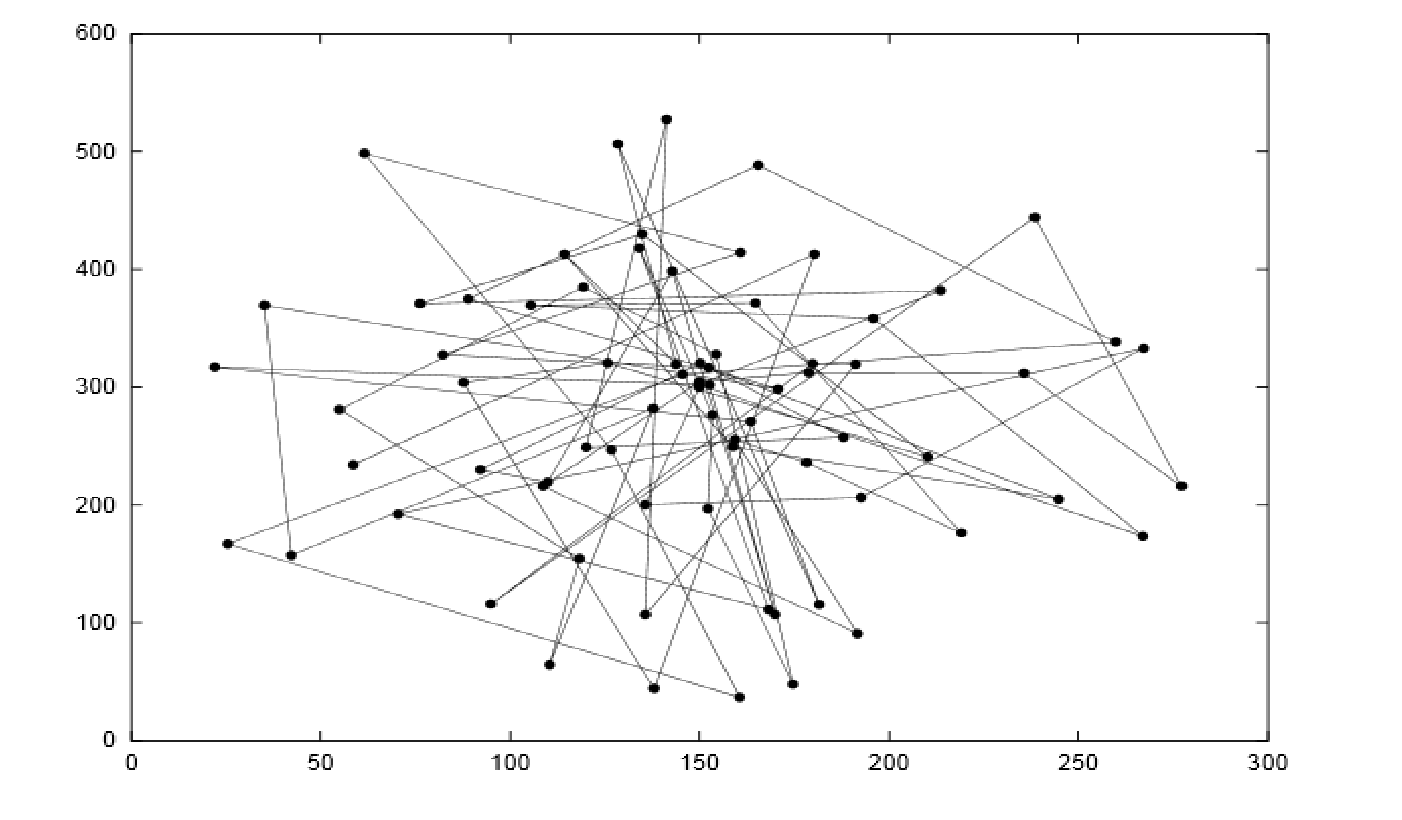
\includegraphics[width=10cm,height=55mm]{../images/randomwalk1.png}
\caption{\label{RandomWalkFig}Resulting pattern of a MN using the Random Walk Mobility Model}
\end{figure}

\newpage

\subsection{Random Waypoint}

It includes pause between changes in direction and/or speed. Once this pause expires, the MN chooses a random destination and a speed, that is uniformly distributed [minspeed, maxspeed]. The movement pattern of a MN which uses the RWaypointMM is similar to the RWalkMM if pause time is zero and [minspeed, maxspeed] = [speedmin, speedmax]. Figure \ref{RandomWaypointFig} shows an example of the resulting pattern from the Random Waypoint Mobility Model.\\

\begin{figure}[h]
\center
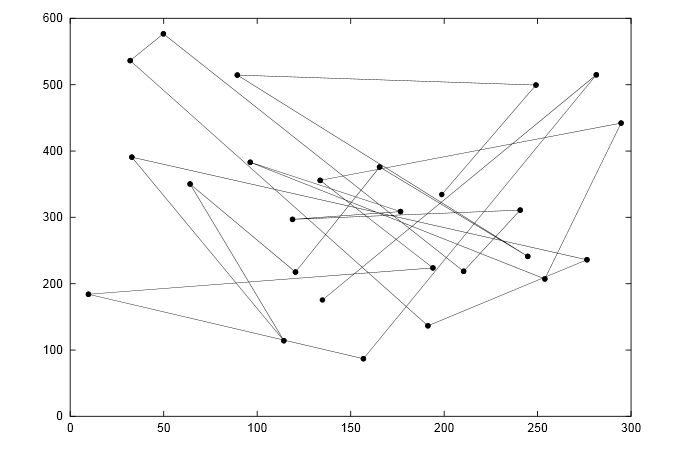
\includegraphics[width=10cm,height=55mm]{../images/randomwaypoint1.png}
\caption{\label{RandomWaypointFig}Resulting pattern of a MN using the Random Waypoint Mobility Model}
\end{figure}

During a run, MNs are initially distributed randomly around the simulation area. Figure \ref{RandomWaypointFig2} shows the average MN neighbors percentage of the MNs. The average is the cumulative percentage of total MNs that are a given MN's neighbor. Therefore, if the network has 20 nodes and a node has 2 neighbors, then the node's current neighbors percentage is 10\%. Moreover, during the first 600 seconds, due to initially distributed randomness of the MNs around the simulation area, there is an high variability in the average MN neighbors percentage.\\
In the paper, three possible solutions are presented to avoid this initialization problem. The first is to save the location of the MNs after the initial high variability and use this position as the initial starting point of the MNs in the next simulations. The second is to change the initial distribution of the MNs in a specific area to be a distribution more common the model, like for example, initially placing the MNs in a triangle distribution. Lastly, the beginning of each simulation produces initialization problems due to the random distribution of the MNs around the simulation area. Throwing out the initial 1000 seconds of simulation time in each simulation ensures that the initialization problem is removed even if the MNs moves slowly. But if the MNs moves fast, we can discard fewer seconds of simulation time. This third solution ensures that each simulation has a random initial configuration.\\

\begin{figure}[h]
\center
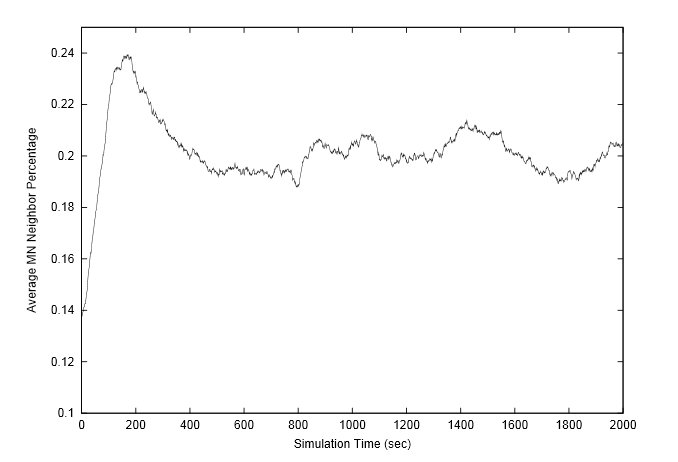
\includegraphics[width=10cm,height=55mm]{../images/randomwaypoint2.png}
\caption{\label{RandomWaypointFig2}Average neighbor percentage vs. time}
\end{figure}

\newpage

\subsubsection{Random Direction}

The Random Waypoint Mobility Model produces a clustering of nodes near the center of the simulation area (see the figure \ref{RandomWaypointFig}). To overcome this problem, the Random Direction Mobility Model was created to ensure an almost constant number of nodes throughout the area simulation.\\ 
In this model, a Mobility Nodes (MNs) chooses a random destination and it will travel to this in order to reach the border of the simulation area. When a MN reaches a simulation boundary, it pauses for a time specified by the simulation. Then it chooses an other angular direction between 0 and 180 degrees and continues to travel.\\ 
Figure \ref{RandomDirectionFig} shows us the resulting path of an MN using this mobility model. This MN begins at the center of the area(150,300). The dots in this figure illustrate the moment when a MN reached a border, paused and chose a new direction to travel along.\\

\begin{figure}[h]
\center
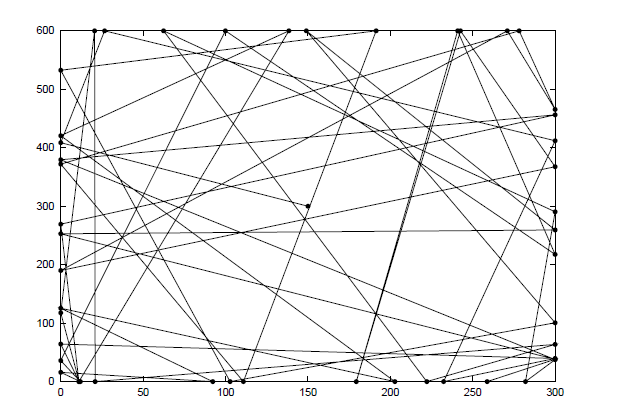
\includegraphics[width=10cm,height=55mm]{../images/randomdirection1.png}
\caption{\label{RandomDirectionFig}Resulting pattern of a MN using the Random Direction Mobility Model}
\end{figure}

\newpage

\subsubsection{A Boundless Simulation Area}

In this model, there is an important relationship between the old direction and velocity and the current direction and velocity. A velocity vector V = (v,theta with v a speed and theta an angular) is used to describe an MN's velocity and a position of an MN is represented as (x,y). The velocity vector and the position are updated in a regular time t.\\
The Boundless Simulation Area Mobility Model is very different from other Mobility Models because here, an MN that reached a border of the simulation area continues its travel and reappears on the opposite side of the simulation area. It results from this that we can consider the simulation area like a torus-shape, illustrated by figure \ref{BoundlessFig}. The simulation area is transformed in two steps. Firstly, the top border is connected to the bottom border to create a cylinder and then we connected both open circular ends.\\

\begin{figure}[h]
\center
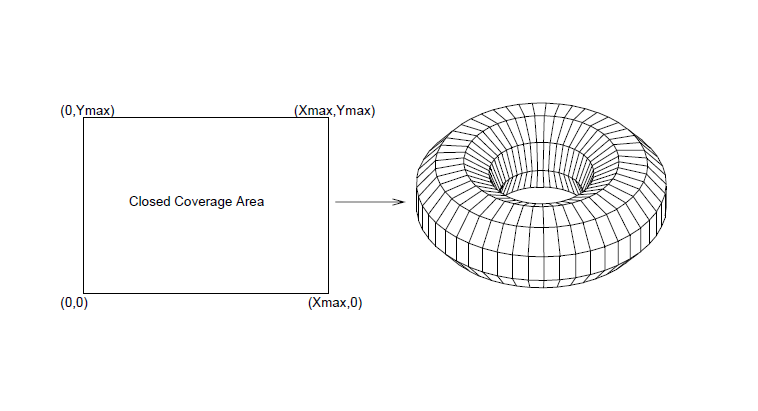
\includegraphics[width=10cm,height=55mm]{../images/boundlessmobilitymodel1.png}
\caption{\label{BoundlessFig}Area mapped to a torus}
\end{figure}


With a speed between 0 and 10 m/s, an angular between 0 and 90 degrees and a time t to 0.1 seconds, the results of the boundless mobility models with this parameters can be seen on figure \ref{BoundlessFig2}\\

\begin{figure}[h]
\center
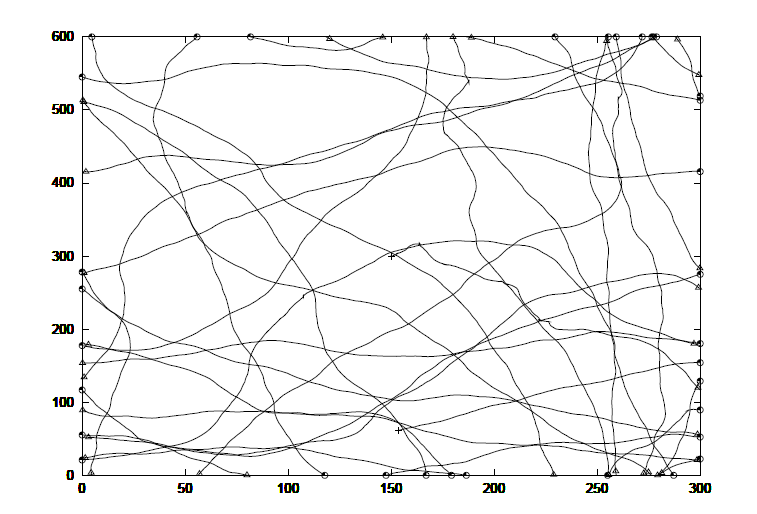
\includegraphics[width=10cm,height=55mm]{../images/boundlessmobilitymodel2.png}
\caption{\label{BoundlessFig2}Resulting pattern of a MN using the Boundless Simulation Area Mobility Model}
\end{figure}

\newpage

\subsection{City section}

The aim of this model is to propose a realistic model. It is based on the vehicle's movement on road maps. The specificity of this model is the map which depends on each geographical zone. Here, vehicles are mobile nodes.\\

The mapping data blocks are available from the Americans office of census. The map information is retrieved from text files. These files are composed of several elements:

\begin{itemize}
\item The unique identifier for a specified road.
\item The nature of the road: it can be a highway or a street.
\item The longitude of the start of position.
\item The latitude of the start of departure
\item The latitude of arrived.
\item The longitude of arrived.
\end{itemize}

All the intersections of the map are represented by nodes not mobile.
This model also considers the volume of traffic : the more there is traffic, the thicker the line representing the road.
This model is also sensitive at the speed of cars (depending in particular on the hour). For example, we can consider that the speed of vehicular traffic in the morning is much smaller than at the beginning of the afternoon.\\

Here is the progress of this model. Every node begins in a point chosen randomly and its destination is chosen also randomly. The strategy of every node is to look for the shortest up to the destination. To achieve it, the Dijsktra algorithm is used. Several parameters have to be considered in this algorithm as the speed or the traffic. This route can be dynamically changed. When a node reaches its destination, it begins again all the process described previously. Concerning the node's speed, it is limited to more or less 5\% of the speed registered in the file.\\
For example, here is a representation of the model. We see here that the traffic is a little sparse, but with very different speeds. The comparisons of these two regions base themselves on the inaccessible pairs, the length of the average route and to finish the changes of neighbors.\\

This article proposes two situations.
The first situation, which they call region A, proposes a very dense road network with a constant speed limit on all the road network. The second situation, which they call region B, proposes a road network much less dense than the precedent, but with different speeds of movements.

The comparisons of these two regions base themselves on the inaccessible pairs, the length of the average route and to finish the changes of neighbors.\\

Here are representations of these two regions:\\

\begin{tabular}{cc}
   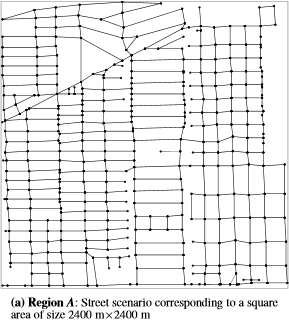
\includegraphics{../images/cityA.png} &
   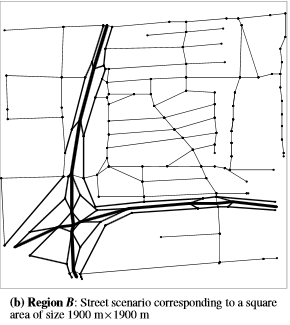
\includegraphics{../images/cityB.png}
\end{tabular}

\newpage

\begin{multicols}{2}
\textit{\textbf{Région A}}
\begin{itemize}
\item Transmission range : 250 meters.
\item 200 nodes.
\item 10\% of the pairs of nodes are unable to communicate.
\item the connectivity of a network is poor
\item New parameters : Transmission range : 500 meters.
\item 50 nodes.
\item Result : the connectivity fluctuates a lot.
\end{itemize}
\columnbreak
\textit{\textbf{Region B}}
\begin{itemize}
\item Transmission range : 250 meters.
\item 200 nodes.
\item 5\% of the pairs of nodes were disconnected.
\item Result: The connectivity is better than in the region A.
\item New parameters : Transmission range : 500 meters.
\item 50 nodes.
\item The area covered in Region B is less than the area covered in Region A.
\item The connectivity corresponding to Region B is better as compared to scenarios corresponding to Region A.
\end{itemize}
\end{multicols}

Another experiment was conducted on the two regions previously mentioned with a routing protocol called DSR. The DSR protocol consists of two mechanisms : Route Discovery and Route Maintenance. According to the article, 
\begin{quotation}
To perform a Route Discovery for a destination node D, a source node S broadcasts a ROUTE REQUEST that gets flooded through the network in a controlled manager. This request is answered by a ROUTE REPLY from either D or some other node that knows a route to D. To reduce frequency and propagation of ROUTE REQUESTs each node aggressively caches source routes that the node learns or overhears.\\
Route Maintenance detects when some link over which a data packet is being transmitted breaks\cite{VehicularAdHocNetworks9}.
\end{quotation}

Simulations were made by using 150 nodes with a wireless transmission range of 500m. The communication  pattern  consisted of 10 constant bit rate flows, each sending 4 64 Bytes data packets from the source to the destination.
The evaluation of this protocol is made on 3 properties.

\begin{itemize}
\item Packet Delivery Ratio
\item Packet delivery latency
\item Packet overhead
\end{itemize}

Here are the results obtained with the DSR protocol:\\

\begin{figure}[h]
\center
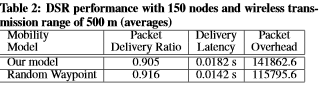
\includegraphics{../images/protocoleDSR.png}
\caption{\label{ProtDSR}DSR Performance}
\end{figure}

We see that the obtained results are very similar in the Waypoint model. The average path length does not differ much.\\
We can conclude that from it the Waypoint model is a very good approximation of the model concerning streets.\\
Numerous improvements are possible so that the model is realistic :

\begin{itemize}
\item Changing settings depending on the time (lots of car in the morning for example).
\item Possibility of introducing obstacles.
\item Currently, each vehicle moves independently. But in real life, it has to pay attention to its environment.
\item The model does not take into account the waiting time in the intersections.
\end{itemize}

To conclude, this model uses real life data. A called  DSR protocol was used to test the model. We were able to notice that the Waypoint model is a good approximation of the model concerning streets.

\newpage

\subsection{Gauss-Markov}

The aim of this model is to be able to adapt with one parameter to different levels of randomness.\\
Each MN has a current speed and direction. The speed and direction of each MN are updating at a regular time t. At each time t, the next destination and speed are calculated based on the current position of the MN. The MNs are forced away from an edge when the location of a MN is near a border of the simulation area, by modifying the angular direction of the MN as illustrated in figure \ref{Gauss-MarkovFig1}.\\

\begin{figure}[h]
\center
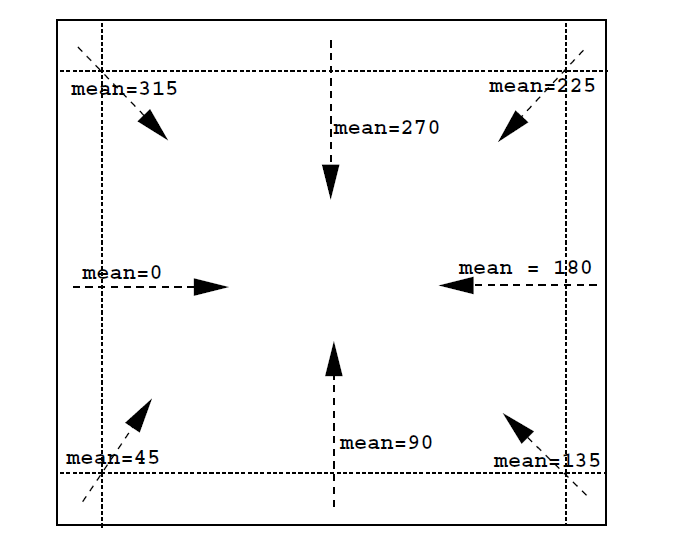
\includegraphics[width=10cm,height=55mm]{../images/gauss-markovmodel1.png}
\caption{\label{Gauss-MarkovFig1} Change of angular direction near a border}
\end{figure}

In figure \ref{Gauss-MarkovFig2}, an example of a resulting pattern of a MN using the Gauss-Markov Mobility Model is illustrated. The run takes 1000 seconds and the MN beings at the center of the simulation area. The parameter t is 1 second, the initial angular is 90 degrees and the speed is between 0 and 10 m/s. The Gauss-Markov MM can eliminate the sudden stops and sharp turns encountered in the Random Walk Mobility Model by saved past velocities and directions in order to be able to influence future velocities and directions.\\

\begin{figure}[h]
\center
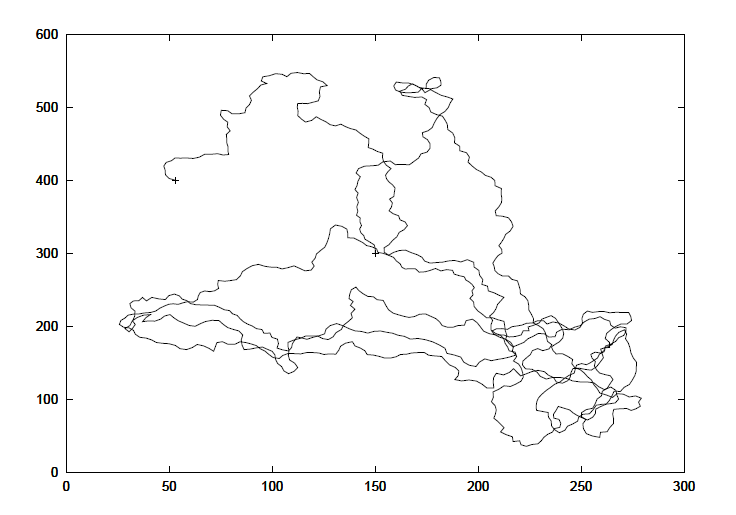
\includegraphics[width=10cm,height=55mm]{../images/gauss-markovmodel2.png}
\caption{\label{Gauss-MarkovFig2} Traveling pattern of an MN using the Gauss-Markov Mobility Model}
\end{figure}

\newpage

\subsection{Reference Point Group Mobility Model}

Group movements are based on the movement at the center of the group. The movement of the group center completely characterizes the motion of the MNs of its group, including their direction and speed. Each MN randomly and individually moves about their own pre-defined reference points, where their movements depend on the group movement. Their position are regularly updated each time t and a new direction is calculated for every MN according to the center of the group.\\
The figure \ref{RPGMMFig} shows us an illustration of a group of three MNs that move together. The Random Waypoint Mobility Model is used for the random motion of each individual MN in the group and the movement at the center of the group.\\
In the paper, an application of this model is explained. The RPGMM can be used for example in an avalanche rescue scenario. In a scenario like this, the cooperation between human and canine is essential. We can see the human as the center of the group and the dogs are the MNs of the group.\\

\begin{figure}[h]
\center
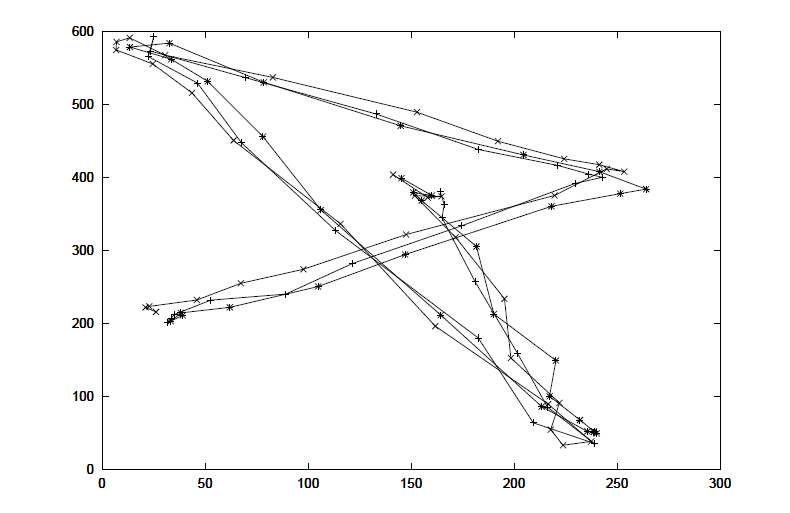
\includegraphics[width=10cm,height=55mm]{../images/rpgmmodel1.png}
\caption{\label{RPGMMFig}Resulting pattern of a MN using the Boundless Simulation Area Mobility Model}
\end{figure}

\newpage

\subsection{Social Network Theory}

This model is based on the theory of social networks and on the decisions and the social behavior of human beings. For example, how human beings move in a group, and between groups. A notion of relation between the people is thus identified.\\
In this model, the individuals and the groups of individuals are considered as entities of the first one classes. The second class represents the strength of the social links (probability of collocation).\\

Representation of social networks is made through weighted graphs, by defining the weights associated with each edge of the network to model the strength of direct interactions between individuals. The degree of interaction is a value between 0 and 1. 0 represents no interactions, 1 represents a strong interaction.
The model assumes a level of interaction less than 0.25 represents a social interaction disconnection.\\

\begin{figure}[h]
\center
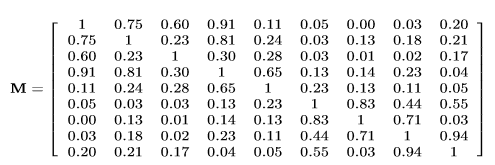
\includegraphics{../images/MatrixInteractionSocialNetwork.png}
\caption{\label{MatricSN}Matrix of interactions between nodes}
\label{MatricSN}
\end{figure}

The objective of this model is to use social relationships between the individuals to define groups of hosts who move together along with the scenarios.
The first step is the generation of the social network. It is represented by a matrix of interaction \pageref{MatricSN}.\\

People can be grouped according to their social links or compared with their geographical location. Dynamic mechanisms are present in this model. The people can belong to a group at moment T, and change group afterward. The notion of distance is taken into in account in the parameters.\\
An incalculable number of scenarios can be set up. Every group moves with a random speed and every host has a random speed of its own. A host, belonging to a group, moves inside this one. He can reach for example an aim which was fixed to its. Nodes not belonging to any group move randomly.\\

When a node reached its aim, it has to make a choice:
either it stays in the group to which it is up, or
it chooses to be alone.
This choice is made according to the rate of sociability of the group.The node will join the group which exercises most attraction.\\

Two scenarios are presented for this model. They are characterized by a number of different nodes and a different number of groups.  The zone of simulation is a square of 1km on 1km, the zone of a group is of 200m. Every group has a speed between 1 and 2 m/s and every node has a speed between 1 and 3 m/s. The first scenario includes 30 computers (representing nodes) consisted in 5 geographically different groups. The second scenario includes 60 computers distributed in 5 groups. In both cases, 80\% of nodes are in a group. Thanks to these scenarios, we can obtain the average degree of connectivity of this model.\\

\begin{tabular}{cc}
   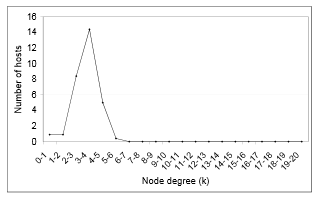
\includegraphics[scale=0.7]{../images/degreeConnectivitySocialNetwork30Nodes.png} &
   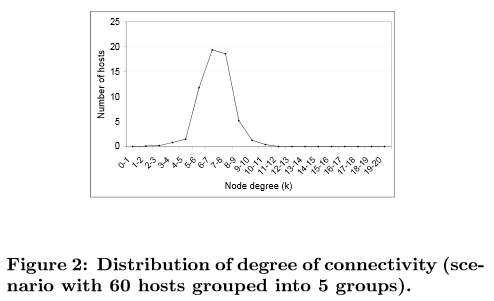
\includegraphics[scale=0.6]{../images/degreeConnectivitySocialNetwork60Nodes.png} \\
\end{tabular}

In conclusion, as regards this model, we can say that generally, the models of existing mobility leans on random movements which are very simplistic and most of the time unrealistic. It is necessary to make models which base themselves on real elements. Here, it is human socialization which is put forward. But this model can still be improved for example by adding obstacles.

\newpage

\subsection{Pheromone}

\subsubsection{Description of the model}

This model is inspired by real pheromone. A pheromone is a chemical substance, secreted externally by certain animals, such as insects, affecting the behaviour or physiology of other animals of the same species.\footnote{\url{http://dictionary.reference.com/browse/pheromone?s=t}}\\
This model use digital Pheromone.This pheromone has 3 properties :

\begin{itemize}
\item  Deposited and withdrawn pheromone from an area. (Information fusion and aggregation).
\item  Evaporated over time. (Forget old information = Truth maintenance).
\item  Propagated from a place to its neighboring places. (Information diffusion and dissemination). 
\end{itemize}

A  digital  pheromone  represents  information  about  the  system. Different  "flavors"  of  pheromones convey different kinds of information.\\ We can have for example, attractive pheromone or repellent pheromone. The attractive pheromone will attract other UAVs whereas the repellent pheromone will repulse other UAVs. Digital pheromones exist within in an artificial space called a pheromone map.

\newpage

\subsubsection{Scenario possible}

Pheromone logic  can  be  used  for  several  types  of  surveillance  and target  acquisition  and  tracking scenarios.\\

\begin{itemize}
\item Surveillance and Patrol

\begin{figure}[h]
\center
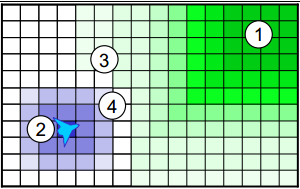
\includegraphics[scale=0.7]{../images/pheromone_surveillance.png}
\caption{\label{surveillance}Attractive and repulsive pheromones for surveillance}
\end{figure}

In Figure \ref{surveillance}, each step mean :\\
 1. Surveillance area deposits attractive pheromone,\\
 2. UAV deposits repulsive pheromone,\\ 
 3. Pheromone infrastructure propagates both attractive and repulsive pheromone to form gradient,\\
 4. UAV climbs net gradient, withdrawing attractive pheromone.
 
\item Target Acquisition

\begin{figure}[h]
\center
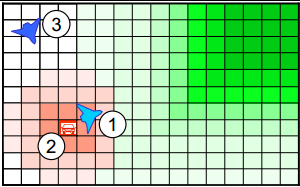
\includegraphics[scale=0.7]{../images/pheromone_target_acquisition.png}
\caption{\label{targetacquisition}Pheromones attracting confirming sensors}
\end{figure}

In Figure \ref{targetacquisition}, each step mean :\\
1. UAVdet detects target and Red target is created,\\
2. Red target deposits “NeedsID” pheromone, \\
3. UAVid is more attracted to NeedsID pheromone than lawn pheromone and climbs gradient to ID target.

\newpage

\item Target Tracking

\begin{figure}[h]
\center
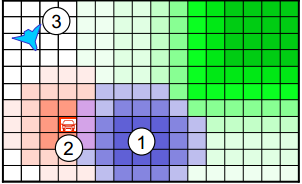
\includegraphics[scale=0.7]{../images/pheromone_tracking.png}
\caption{\label{tracking} Pheromone tracking algorithm}
\end{figure}

In Figure \ref{tracking}, each step mean :\\
1. UAV acquires target and large Visited pheromone deposit repelling 
other UAVs,\\
2. Red target estimates movement, deposits “Tracking” pheromone that eventually overcomes strength of Visited pheromone, \\
3. Nearby UAV is more attracted to Tracking pheromone than repelled by Visited pheromone and climbs gradient to reacquire the target. 
\end{itemize}

\newpage

\subsubsection{Real scenario}

We are going to see a real scenario which demonstrate the use of pheromone model.\\
The demonstration used: 

\begin{itemize}
\item Four robots 
\item A mock urban area  
\item Two UAVs controlled by pheromone technology 
\end{itemize}

The demonstration focused on the swarming algorithms that control and coordinate the behaviors of the heterogeneous mix of vehicles.\\
Pheromone  algorithms  controlled  and  coordinated  the  flight  of  the  two  UAVs  as  they performed continuous  surveillance  over  an  urban  area  looking  for  potential  adversaries. The  two  air  units worked together to ensure even, thorough, and continuous coverage of all areas in the surveillance region  while  avoiding  any  collisions. They  also  provided  patrol coverage  of  a  mock  convoy  as  it moved through the area.\\ 
While the UAVs surveyed a broad area over the airfield, the ground robots surveyed and patrolled around  some  mock  buildings  set  up  for  the  demo.\\
During  the  demonstration,  one  of  the  ground robots  failed. The  other  ground  robots were  able  to  dynamically  readjust  their  patrol  patterns to accommodate  the  missing  unit without  any  intervention  by  the  operator.\\
This  unplanned  event helped to demonstrate the robustness of these algorithms to unexpected events. The  demonstration  showed  cooperative  behavior  between  the  air  and  ground  units when  the identity of a potential adversary detected by one of the UAV’s was automatically confirmed by one of the ground robots with a special sensor capable of target identification.\\
The operator simply gives a high level command to the whole swarm, such as “survey this area and track  any  identified  targets”  or  “patrol  around  this  convoy”.\\
The  robots  autonomously  configured themselves to determine which robot would perform what task in order to accomplish the overall objective.

\newpage

\subsection{Natural Agent}

The basic idea of this article is the simulation of mobile model by basing itself on animal behavior.
Animals, called a mobile agent in the article, cannot be separated from the environment in which they are and through which they interact. This idea is often ignored in the works on computer multi-agent systems, or the researchers consider the environment as a communication framework liability.\\
A multi-agent system is a three-tuple : 

\begin{itemize}
\item a set of agents,
Each agent, which is a four-tuple constitued of : 
\begin{itemize}
\item a set of agent,
\item a state, 
\item an input 
\item and an output(subset of state)
\end{itemize}
\item an environment. 
\item and a process which allows to change the state of the agent.
\end{itemize}

The presence of input and output shows that the agents are limited processes : Environment, and a coupling.\\
The environment is a 2-tuple which is a subset of an agent.\\
It has a state and a process.\\ 
The environment is active. It has its own process which can change its state. The works on the artificial agents lean on the artificial intelligence. None agents only can predict the effect of its actions on the environment, because they do not depend on an agent but of a set of agent.\\
Thereafter, we are going to describe you the different mobile agents described in this article.

\newpage

\subsubsection{Ants}

The ants model is based on the fact that ants build networks of paths. These paths link their food source available to their nest.
Each ant who eat has the same program:

\begin{itemize}
\item It must avoid obstacles.
\item If there is no pheromone on the map, it can go where it wants (random trajectory).
\item If it finds some food, it depose pheromone during a time t. These pheromones indicate to other ants the location of the food.
\item If an ant finds some food, it pick them up if it's not holding any and brings back the food to its nest.
\end{itemize}

Ants can die. Either they don't find food enough rapidly, or predators kill them.\\
All pheromone paths link to food. But the pheromones evaporate over time. The rate of pheromone can be reinforced if many ants come through the same path.\\
Here is a representation of the behavior of ants (This diagram is from \url{http://pro.cleamax.fr/info-bioinspiree/?p=fourmis}) :

\begin{figure}[h]
\center
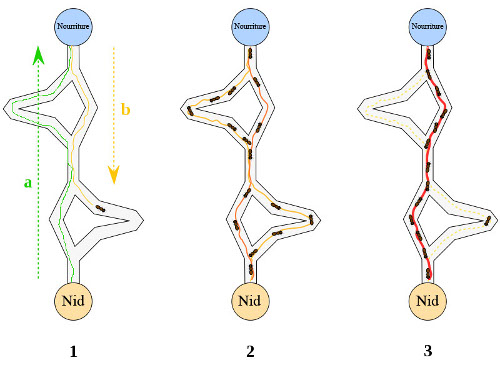
\includegraphics{../images/SchemaFourmi.png}
\caption{\label{AntsRepresentation}Representation of ants}
\end{figure}

\newpage

\subsubsection{Ants: Brod Sorting}

This model is similar to the model previously quoted. It is based on a system of sorting concerning entities. A nest shelters various things inside, larvae, eggs, food. The ant colony keeps the entities sorted by kind.
The behavior of ants goes this way:

\begin{itemize}
\item Ants have a random behavior around the nest.
\item Ants locate nearby objects and memorize them.
\item If an ant was carrying no element, it has the choice to collect the object or to leave it. The probability to collect an object decreases if the ant recently met similar objects.
\item If an ant carries something, it can decide at any time to release this element. The probability that it releases, increases if the ant has recently met similar elements in the environment.
\end{itemize}

\newpage

\subsubsection{Termites}

This model is based on the behavior of termites. These also use pheromones. Here are the rules followed by termites:

\begin{itemize}
\item Pheromones consist of physical waste.
\item This waste is the material from which the termite mound is constructed.
\item If there is no pheromone, ants move in a random way. If they detect pheromones, they will prefer to follow the strongest local pheromone concentration.
\item At each time step, termites decides if they deposit pheromones.
\item The rate of pheromone is decreasing according to time.
\end{itemize} 

\newpage

\subsubsection{Wasps}

The model based on wasps consists of several characteristics:

All the wasps are distributed in three groups.
\begin{itemize}
\item A single chief which distributes the various wasps in various groups.
\item A group of foragers which has the mission to go hunting in order to obtain food.
\item A group of nurses which care for the brood.
\end{itemize}

Every wasp gets three parameters. The first one concerns the strength of the wasp. It also represents the way it moves. The second parameter corresponds to a foraging threshold which determines the probability for a wasp to fetch of the food. The third parameter is associated with the brood. It allows to specify the demand in food. It allows to stimulate the foragers.\\
When two wasps meet, they are engaged in a fight.
The winner of the fight is designated according to the strength of each wasp. Moreover, the demand of broods in food decreases if they have recently received.

\newpage

\subsubsection{Birds and Fish}

This model is based on flocks of birds and schools of fish, which present the same coordinated behavior.\\
Indeed, they can turns together and avoid collisions with obstacles and between each others.\\

The human societies address similar problems, in air-traffic control and convoys of ships, but the human solutions depend on sophisticated communication an central coordination structures not available to birds and fish.\\

So, in order to answer to these troubles, the model follow three simple rules.
\begin{itemize}
\item maintain a specified minimum separation from the nearest object or neighbor,
\item match magnitude and direction to nearby neighbor,
\item and stay close to the center of the flock.
\end{itemize}

The flock or school is a self-constraining structure in which each entity’s individual
actions simultaneously respond to and change the overall structure of the flock. Although each bird or
fish senses only the movements of its nearest peers, its responses to these movements propagate to
others, so that the system as a whole exhibits global coordination.\\

\newpage

\subsubsection{Wolves}

This model is based on the communication of wolves in order to hunt mooses.\\
The system behavior is simple. A single wolf, cannot kill a moose, because of his larger and powerful hooves.\\
So, in order to hunt him, pack of wolves, must first surround the moose, so that one can jump on it's backs, while it is occupied with the others.\\

The problem is how to modelized this behavior ?\\
In fact, it's seems simple for us. For example, Human SWAT teams use radio to coordinate such surrounding maneuvers, but wolves don’t have walkie-talkies or similar long-range communication mechanisms.\\

So, this model was for many years a major problem in the field of distributed artificial intelligence, known as "predator-prey" problem.\\

Many of the proposed solutions assumed reasoning and communication capabilities whose existence in wolves is doubtful at best. For example, the emulated wolves would communicate and negotiate their strategies with one another (“I’ll head for the north side; why don’t you go to the south?”).\\
Finally, a simpler solution requires only rudimentary sensing and action on the part of both moose and wolves.\\
These actions are emulated on a hexagonal grid, six wolves will always capture the moose (with one wolf on each cell adjacent to the moose’s cell) as long as it cannot run faster than them.\\

The solution follow two points :
\begin{itemize}
\item The Moose move to the neighboring cell that is farthest away from the nearest wolf. As long as its rate of movement is faster than that of the wolves, this strategy permits it to escape.
\item Wolves move to the neighboring cell with the highest score
\end{itemize}

The score of a cell is compute with this equation :
\begin{lstlisting}[frame=trBL, title=Score calculation]
			S = d(moose)-k*d(wolf)
\end{lstlisting}
~\\
where d(moose) is the distance to the moose, d(wolf) is the distance to the nearest other wolf, and k is a
tuning constant, modeling a repulsive force between wolves.\\

As in the example of birds and fish, each entity in the wolf-moose system both influences and is influenced by the entire system.\\
Behavior of the overall system depends critically on the relative speeds of moose and wolves, and on the value of the parameter k that establishes the repulsion among wolves. When repulsion and attraction are suitably balanced, the wolves inevitably surround the moose, without any explicit communication or negotiation of strategies.
